\appendix
\backupbegin
\section{Appendix}

\subsection{Meta Model}
\begin{frame}
\frametitle{The Activity Test Case Graph Model}
	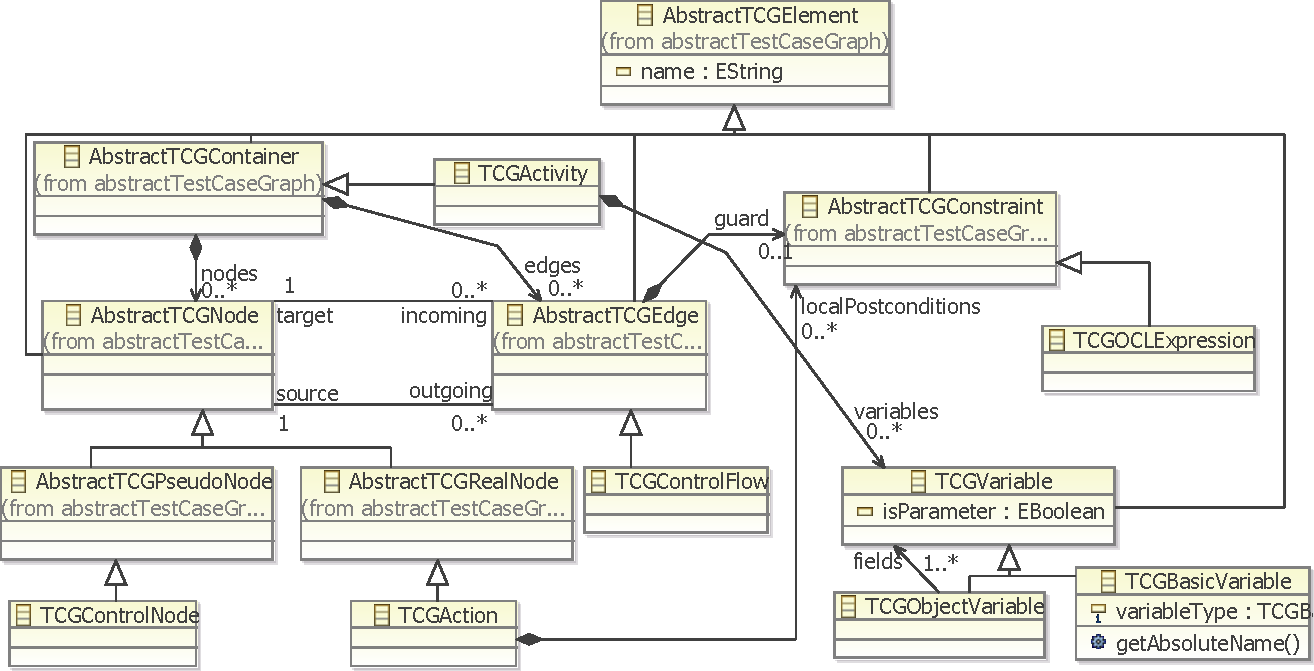
\includegraphics[width=\textwidth]{../IntermediatePresentation/pics/completeMetamodelforSlideshowN.pdf}
\end{frame}

\subsection{Solvers}

\begin{frame}
\frametitle{Expressiveness and Complexity of Constraint Languages}
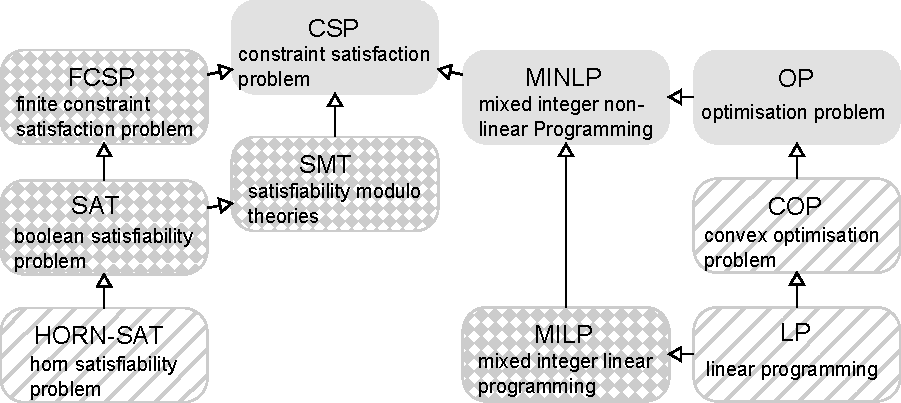
\includegraphics[width=\textwidth]{pics/ProblemLatice.pdf}
\end{frame}

\begin{frame}
\frametitle{Tested Solvers}
\begin{center}
\begin{tabular}{l r r r r r r r r}
Solver & LP & MILP & COP & OP & SAT & SMT & FCSP & MINLP\\
\hline
Cplex & \checkmark & \checkmark & & & & & &\\
IlogCP & \checkmark & \checkmark & & & \checkmark & \checkmark & \checkmark &\\
GeCoDE & & & & &\checkmark & \checkmark & \checkmark &\\
JaCoP & & & & &\checkmark & & \checkmark &\\
Couenne & \checkmark & \checkmark & \checkmark & \checkmark & & & & \checkmark\\
Gurobi & \checkmark & & \checkmark & & & & &\\
LPsolve & \checkmark &\checkmark  & & & & & &\\
Minos &\checkmark & &\checkmark & & & & &\\
% conopt & & & & & & & &\\
% knitro & & & & & & & &\\
% snopt & & & & & & & &\\
% xpress & & & & & & & &\\
% bonmin & & & & & & & &\\
% cbc & & & & & & & &\\
% ipopt & & & & & & & &\\
\hline
\end{tabular}\end{center}
\end{frame}

\subsection{Binary Counter}
\begin{frame}
\frametitle{Binary Counter}
% \def\svgwidth{\textwidth}
% \scriptsize
% \input{./pics/TriangleClasificator.pdf_tex}
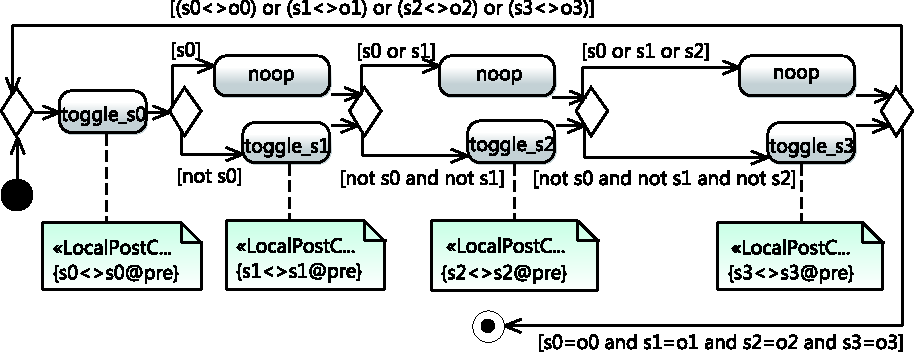
\includegraphics[width=\textwidth]{./pics/BinaryCounderSMT.pdf}
\end{frame}


\begin{frame}
\frametitle{Runtime Measurement for Different Solvers}
\begin{tikzpicture}
\begin{axis}[
width=0.598\textwidth,
height=7.5cm,
xlabel={maximum path length},
ylabel={time $[s]$},
legend style={legend columns=1,at={(0.02,0.98)},anchor=north west},
%yticklabels={0,{$1$},{$10$},{$100$},{$10^3$},{$10^4$},{$10^5$}},
extra y ticks={3.6e12,2.592e14},
extra y tick labels={{1h},{3d}},
extra tick style={
        major grid style=black,
        tick align=outside,
        tick style=black
    },
minor x tick num=1,
ymajorgrids=true,
yminorgrids=true,
xmajorgrids=true,
xminorgrids=true,
ymode=log,
xmin=5,
xmax=95,
]
\addplot[blue,no markers] table[x=PATHSEARCH_MAX_PATHLENGTH,y=time(ns)]{../Thesis/Experiment-DATA/BinaryCounterGecode+presolveSMT.csv};
\addlegendentry{GeCoDE};
\addplot[red,no markers] table[x=PATHSEARCH_MAX_PATHLENGTH,y=time(ns)]{../Thesis/Experiment-DATA/BinaryCounterJacop+presolveSMT.csv};
\addlegendentry{JaCoP};
\end{axis}
\end{tikzpicture}%
\begin{tikzpicture}
\begin{axis}[
width=0.398\textwidth,
height=7.5cm,
nodes near coords,
xmin=5,
xmax=95,
% xtick={10,20,30,40,50,60,70,80,90},
xlabel={maximum path length},
ylabel={total number of test cases},
]
\addplot+[black,mark=x,only marks] table[x=PATHSEARCH_MAX_PATHLENGTH,y=PathsFound]{../Thesis/Experiment-DATA/BinaryCounterGecode+presolveSMT.csv};
\end{axis}
\end{tikzpicture}
\end{frame}

\subsection{Case Study}
\begin{frame}
\frametitle{Runtime Depending on the Number of Test Cases}
\begin{tikzpicture}
\begin{axis}[
width=\textwidth,
height=7.5cm,
legend style={legend columns=1,at={(0.02,0.98)},anchor=north west},
xlabel={number of test cases},
ylabel={time $[s]$},
scaled y ticks = false,
% xtick scale label code/.code={\xdef\xtickscale{#1}}, 
yticklabels={0,{$1$},{$10$},{$100$},{$10^3$},{$10^4$},{$10^5$}},
extra y ticks={3.6e12,2.592e14},
extra y tick labels={{1h},{3d}},
extra tick style={
        major grid style=black,
        tick align=outside,
        tick style=black
    },
minor x tick num=1,
ymajorgrids=true,
yminorgrids=true,
xmajorgrids=true,
xminorgrids=true,
ymode=log,
xmode=log,
] 
\addplot[red] table[x=PathsFound,y=time(ns)]{../Thesis/Experiment-DATA/CaseStudyRuntimeBFS.csv};
\addlegendentry{breadth first search (Cplex)}
\addplot[green] table[x=PathsFound,y=time(ns)]{../Thesis/Experiment-DATA/CaseStudyRuntimeCplex.csv};
\addlegendentry{depth first search (Cplex)}
\addplot[blue] table[x=PathsFound,y=time(ns)]{../Thesis/Experiment-DATA/CaseStudyRuntimeLPSolve.csv};
\addlegendentry{depth first search (LPSolve)}
\addplot[color=black, style=dashed] expression[no markers, domain=1e2:1e5]{(2e7) * x}
node [pos=0.7,below,sloped,fill=white,opacity=0.85,text opacity=1] {$x^1$} 
;
\addplot[color=black, style=dashed] expression[no markers, domain=1e2:1e5]{(4e6) * x ^ (1.45)} 
node [pos=0.9,sloped,above,fill=white,opacity=0.85,text opacity=1] {$x^{1.45}$} 
;
\addplot[color=black, style=dashed] expression[no markers, domain=1e2:1e4]{(6e5) * x ^ (2)} 
node [pos=0.7,sloped,above,fill=white,opacity=0.85,text opacity=1] {$x^{2}$} 
;
\end{axis}
\end{tikzpicture}%
\end{frame}

\subsection{Algorithm}
\begin{frame}
\frametitle{Overview of the Algorithm}
\begin{block}{}
Map UML/OCL to simplified intermediate representation.
\end{block}
\begin{block}{}
Transform activity diagram into an AMPL model.
\end{block}
\begin{block}{}
Find control flow paths using depth first search with early infeasible path elimination.
\end{block}
\begin{block}{}
Solve constraint satisfaction problem for each control flow path.
\end{block}
\begin{block}{}
Output test cases as C++ unit tests using the Boost test library.
\end{block}
\end{frame}

\begin{frame}
\frametitle{Goals of Normalisation}
\begin{itemize}
  \item Ensure that the algorithm does not run into error conditions
  \item Slice relevant parts out of a huge UML model
  \item Parse embedded OCL constraints and ensure that they comply to the handled OCL subset
  \item Make implicit constraints automatically explicit
\end{itemize}
\begin{block}{}
Subsequent steps are completely independent from the UML/OCL model
\end{block}
\end{frame}

%\subsection{Abstract Test Case Generation}
\begin{frame}
\frametitle{Abstract Test Case Generation}
\begin{itemize} 
\item Determine appropriate test scenarios fulfilling model structure based coverage criteria
\item Simple breadth first or depth first search used to find control flow paths
\item Maximum path length or number of control flow paths parameter ensures termination of the algorithm
\item Infeasible paths are eliminated by solving all constraints along a path
\item How often infeasible path elimination is performed can be controlled by the parameter unchecked steps
%\item Infeasible paths elimination is performed whenever search is currently examining a real decision node and unchecked steps decision nodes have already been passed without a check
\end{itemize}
\end{frame} 


%\subsection{Specific Test Data Generation}

\begin{frame}
\frametitle{Specific Test Data Generation}
\begin{itemize} 
\item For each test scenario input data and oracle values need to be computed
\item Control flow path is symbolically executed and encoded in AMPL data
\item State--of--the--art constraint solver generates test input and the oracle value from the AMPL program
\item Boundary value analysis is possible by adding an objective function to the AMPL model
\item All generated test data is stored in a language independent unit test model
\end{itemize}
\end{frame}

%\subsection{Unit Test Synthesis}
\begin{frame}
\frametitle{Unit Test Synthesis}
\begin{itemize} 
\item Output compileable unit test code
\item Support state--of--the--art testing framework
\item Model-to-Text transformation from unit test model and activity test case graph
\item Currently C++ unit tests using the Boost test library are generated
\end{itemize}
\end{frame}

\subsection{Atego stuff}
\begin{frame}
\frametitle{Atego\textsuperscript{\textregistered} Artisan Studio Integration}
\begin{itemize}
  \item XMI format exported from Artisan Studio can be imported in Eclipse Modelling Framework.
\end{itemize}

\includegraphics[width=\textwidth]{./pics/AtegoATCGConversion.pdf}
\begin{block}{}
Better let the Normalisation directly access the Atego\textsuperscript{\textregistered} Model API.
\end{block}
\end{frame}

\subsection{Exploding Tyres}
\begin{frame}
\frametitle{Exploding Tyres (mixed integer non linear)}
% \def\svgwidth{\textwidth}
% \scriptsize
% \input{./pics/TriangleClasificator.pdf_tex}
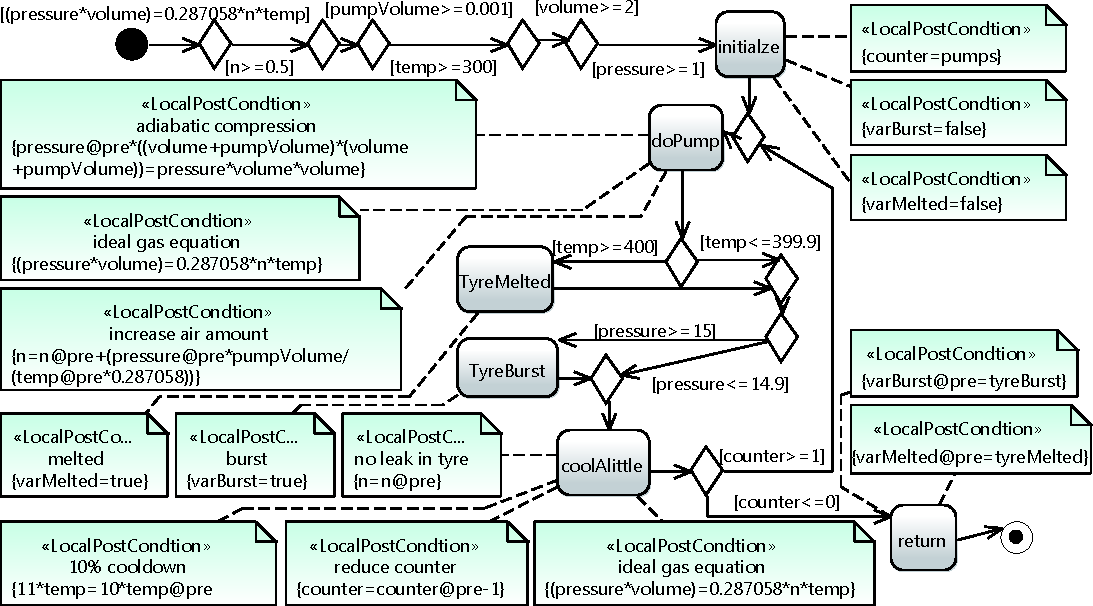
\includegraphics[width=\textwidth]{./pics/TyrePumpModel.pdf}
\end{frame}
\begin{frame}
\frametitle{Runtime with Different Solver Time Limits}
\begin{tikzpicture}
\begin{axis}[
width=0.498\textwidth,
height=7.5cm,
legend style={legend columns=1,at={(0.02,0.98)},anchor=north west},
% legend to name=myLegend,
ylabel={time $[s]$},
xlabel={maximum path length},
yticklabels={{0},{$0.1$},{$1$},{$10$},{$100$},{$10^3$},{$10^4$},{$10^5$}},
extra y ticks={3.6e12,2.592e14},
extra y tick labels={{1h},{3d}},
extra tick style={
        major grid style=black,
        tick align=outside,
        tick style=black
    },
minor x tick num=1,
ymajorgrids=true,
yminorgrids=true,
xmajorgrids=true,
xminorgrids=true,
ymode=log,
xmin=5,
xmax=75,
]
\addplot[blue,no markers] table[x=PATHSEARCH_MAX_PATHLENGTH,y=time(ns)]{../Thesis/Experiment-DATA/ExplodingTyres_10min.csv};
\addlegendentry{10min};
\addplot[red,no markers] table[x=PATHSEARCH_MAX_PATHLENGTH,y=time(ns)]{../Thesis/Experiment-DATA/ExplodingTyres_20sec.csv};
\addlegendentry{20sec};
\addplot[green,no markers] table[x=PATHSEARCH_MAX_PATHLENGTH,y=time(ns)]{../Thesis/Experiment-DATA/ExplodingTyres_5sec.csv};
\addlegendentry{5sec};
% \addplot[dash pattern=on 7pt off 3pt,no markers] table[x=PATHSEARCH_MAX_PATHLENGTH,y=time(ns)]{../Thesis/Experiment-DATA/ExplodingTyres_10s.csv};
% \addlegendentry{10sec};
% \addplot[loosely dashed,no markers] table[x=PATHSEARCH_MAX_PATHLENGTH,y=time(ns)]{../Thesis/Experiment-DATA/ExplodingTyres_60sec.csv};
% \addlegendentry{60sec};
% \addplot[solid,no markers] table[x=PATHSEARCH_MAX_PATHLENGTH,y=time(ns)]{../Thesis/Experiment-DATA/ExplodingTyres_2h.csv};
% \addlegendentry{2h};
\end{axis}
\end{tikzpicture}%
\begin{tikzpicture}
\begin{axis}[
width=0.498\textwidth,
height=7.5cm,
xlabel={maximum path length},
ylabel={number of test cases found},
minor x tick num=1,
minor y tick num=4,
ymajorgrids=true,
yminorgrids=true,
xmajorgrids=true,
xminorgrids=true,
xmin=35,
xmax=75,
]
\addplot[green,no markers] table[x=PATHSEARCH_MAX_PATHLENGTH,y=PathsFound]{../Thesis/Experiment-DATA/ExplodingTyres_5sec.csv};
%\addlegendentry{5sec};
% \addplot[dash pattern=on 7pt off 3pt,no markers] table[x=PATHSEARCH_MAX_PATHLENGTH,y=PathsFound]{Experiment-DATA/ExplodingTyres_10s.csv};
%\addlegendentry{10sec};
\addplot[red,no markers] table[x=PATHSEARCH_MAX_PATHLENGTH,y=PathsFound]{../Thesis/Experiment-DATA/ExplodingTyres_20sec.csv};
%\addlegendentry{20sec};
% \addplot[loosely dashed,no markers] table[x=PATHSEARCH_MAX_PATHLENGTH,y=PathsFound]{Experiment-DATA/ExplodingTyres_60sec.csv};
%\addlegendentry{60sec};
\addplot[blue,no markers] table[x=PATHSEARCH_MAX_PATHLENGTH,y=PathsFound]{../Thesis/Experiment-DATA/ExplodingTyres_10min.csv};
%\addlegendentry{10min};
\end{axis}
\end{tikzpicture}
\end{frame}
\begin{frame}
\frametitle{Mutation Testing the Example Model}
\begin{table}[htb]%
\begin{tabular*}{\textwidth}{@{}l@{\extracolsep{\fill}}*4r}
maximum path length     & 20      & 30      & 40        & 50\\%
\hline%
number of test cases    & 4       & 18      & 47        & 97 \\%
killed mutants          & 553     & 569     & 570       & 573 \\%
alive mutants           & 20      & 4       &  3        & 0 \\%
\hline%
mutation score          & 96.5\%  & 99.3\%  & 99.5\%    & 100\% \\%
\hline%
\end{tabular*}
\label{tab:MutationTesting}%
\end{table}
\end{frame}

\subsection{AMPL Data}
\begin{frame}[fragile]
\frametitle{AMPL Modelling}
	\begin{block}{Specify Path}
		\begin{lstlisting}[basicstyle=\ttfamily\small,language=ampl]
param l := 1;
set d2f:= 0; # guard
set f:= 1; # post condition
		\end{lstlisting}
	\end{block}
	\begin{block}{Result}
		\begin{lstlisting}[basicstyle=\ttfamily\small]
Solution determined by presolve.
a = 5
return = 0
		\end{lstlisting}
	\end{block}
\end{frame}
\backupend

